\documentclass[11pt,a4paper]{article}
\usepackage[utf8]{vietnam}
\usepackage{amsmath,amssymb}
\usepackage{tabularx}
\usepackage{tikz}
\usepackage{xcolor}
\usepackage{fancyhdr}
\usepackage[top=1.8cm, bottom=2.0cm, left=1.8cm, right=1.8cm]{geometry}

\setlength{\parskip}{3pt}
\setlength{\parindent}{0pt}

\pagestyle{fancy}
\fancyhf{}
\renewcommand{\headrulewidth}{0.4pt}
\lhead{\footnotesize \textbf{CHÙA HƯƠNG SƠN -- ÔN THI VÀO 10}}
\rhead{\footnotesize \textbf{ĐỀ THI THỬ CUỐI HỌC KỲ I (ĐỀ SỐ 08)}}
\cfoot{\thepage}

\begin{document}

\noindent
\begin{tabular*}{\linewidth}{@{\extracolsep{\fill}}cc@{}}
\textbf{SỞ GIÁO DỤC VÀ ĐÀO TẠO} & \textbf{ĐỀ KIỂM TRA CUỐI HỌC KỲ I} \\
\textbf{CHÙA HƯƠNG SƠN} & \textbf{NĂM HỌC 2026 -- 2027} \\
\textbf{ĐỀ THI THỬ SỐ 08} & \textbf{MÔN: TOÁN -- LỚP 9} \\
\textit{(Đề thi gồm 03 trang)} & \textit{Thời gian làm bài: 90 phút (không kể thời gian phát đề)} \\
\end{tabular*}

\vspace{2mm}
\noindent
\rule{\linewidth}{0.8pt}

\vspace{1mm}
\noindent
Họ và tên thí sinh: \dotfill Số báo danh: \dotfill

\vspace{2mm}
\noindent
\textbf{\large I. TRẮC NGHIỆM KHÁCH QUAN (7,0 điểm)}

\vspace{1mm}
\noindent
\textbf{Phần 1. Trắc nghiệm nhiều lựa chọn (3,0 điểm).} \textit{Từ câu 1 đến câu 12, thí sinh chọn đáp án đúng nhất trong 4 đáp án A, B, C, D rồi ghi vào bài làm.}

\vspace{1.5mm}
\textbf{Câu 1.} Giá trị của biểu thức $4\sqrt{12} - 3\sqrt{27} + \sqrt{75}$ bằng\\
\begin{tabularx}{\linewidth}{XXXX}
\textbf{A.} $4\sqrt{3}$. & \textbf{B.} $5\sqrt{3}$. & \textbf{C.} $3\sqrt{3}$. & \textbf{D.} $6\sqrt{3}$.
\end{tabularx}

\vspace{1.5mm}
\textbf{Câu 2.} Cho tam giác $ABC$ vuông tại $A$ có góc $\widehat{B} = \beta$. Khi đó $\tan \beta$ bằng\\
\begin{tabularx}{\linewidth}{XXXX}
\textbf{A.} $\dfrac{AC}{AB}$. & \textbf{B.} $\dfrac{AB}{AC}$. & \textbf{C.} $\dfrac{AC}{BC}$. & \textbf{D.} $\dfrac{AB}{BC}$.
\end{tabularx}

\vspace{1.5mm}
\textbf{Câu 3.} Bất phương trình nào sau đây là bất phương trình bậc nhất một ẩn?\\
\begin{tabularx}{\linewidth}{XXXX}
\textbf{A.} $4x - 12 \le 0$. & \textbf{B.} $0x + 8 > 0$. & \textbf{C.} $2x^2 + 3 \ge 0$. & \textbf{D.} $\dfrac{5}{x} - 2 < 0$.
\end{tabularx}

\vspace{1.5mm}
\textbf{Câu 4.} Cho hai số thực $a$ và $b$ thỏa mãn $a < b$. Khẳng định nào sau đây là đúng?\\
\begin{tabularx}{\linewidth}{XXXX}
\textbf{A.} $-3a > -3b$. & \textbf{B.} $-3a < -3b$. & \textbf{C.} $2a + 1 > 2b + 1$. & \textbf{D.} $a - 4 > b - 4$.
\end{tabularx}

\vspace{1.5mm}
\textbf{Câu 5.} Căn bậc hai số học của 196 là\\
\begin{tabularx}{\linewidth}{XXXX}
\textbf{A.} $14$. & \textbf{B.} $-14$. & \textbf{C.} $14$ và $-14$. & \textbf{D.} $38416$.
\end{tabularx}

\vspace{1.5mm}
\textbf{Câu 6.} Điều kiện xác định của căn thức $\sqrt{5 - x}$ là\\
\begin{tabularx}{\linewidth}{XXXX}
\textbf{A.} $x \le 5$. & \textbf{B.} $x \ge 5$. & \textbf{C.} $x < 5$. & \textbf{D.} $x > 5$.
\end{tabularx}

\vspace{1.5mm}
\textbf{Câu 7.} Với mọi số thực $x < 3$, biểu thức $\sqrt{(x-3)^2}$ có giá trị rút gọn bằng\\
\begin{tabularx}{\linewidth}{XXXX}
\textbf{A.} $3 - x$. & \textbf{B.} $x - 3$. & \textbf{C.} $-(3 - x)$. & \textbf{D.} $(x-3)^2$.
\end{tabularx}

\vspace{1.5mm}
\textbf{Câu 8.} Giá trị của biểu thức $\sqrt[3]{-512}$ bằng\\
\begin{tabularx}{\linewidth}{XXXX}
\textbf{A.} $-8$. & \textbf{B.} $8$. & \textbf{C.} $-64$. & \textbf{D.} $64$.
\end{tabularx}

\vspace{1.5mm}
\textbf{Câu 9.} Công thức tính diện tích hình tròn có bán kính $R$ là\\
\begin{tabularx}{\linewidth}{XXXX}
\textbf{A.} $S = \pi R^2$. & \textbf{B.} $S = 2\pi R$. & \textbf{C.} $S = 4\pi R^2$. & \textbf{D.} $S = \pi R$.
\end{tabularx}

\vspace{1.5mm}
\textbf{Câu 10.} Cho đường tròn $(O; 6\text{ cm})$ và đường thẳng $a$. Khoảng cách từ $O$ đến đường thẳng $a$ bằng $4\text{ cm}$. Vị trí tương đối của $a$ và $(O)$ là\\
\begin{tabularx}{\linewidth}{XXXX}
\textbf{A.} Cắt nhau. & \textbf{B.} Tiếp xúc nhau. & \textbf{C.} Không giao nhau. & \textbf{D.} Song song.
\end{tabularx}

\vspace{1.5mm}
\textbf{Câu 11.} Cho hai đường tròn $(O; 7\text{ cm})$ và $(O'; 3\text{ cm})$. Biết đoạn nối tâm $OO' = 10\text{ cm}$. Vị trí tương đối của hai đường tròn là\\
\begin{tabularx}{\linewidth}{XXXX}
\textbf{A.} Tiếp xúc ngoài. & \textbf{B.} Tiếp xúc trong. & \textbf{C.} Cắt nhau. & \textbf{D.} Ngoài nhau.
\end{tabularx}

\vspace{1.5mm}
\textbf{Câu 12.} Trên đường tròn $(O)$, góc ở tâm $\widehat{AOB} = 60^\circ$ chắn cung nhỏ $AB$. Số đo của cung nhỏ $AB$ bằng\\
\begin{tabularx}{\linewidth}{XXXX}
\textbf{A.} $60^\circ$. & \textbf{B.} $30^\circ$. & \textbf{C.} $120^\circ$. & \textbf{D.} $300^\circ$.
\end{tabularx}

\vspace{3mm}
\noindent
\textbf{Phần 2. Trắc nghiệm Đúng -- Sai (2,0 điểm).} \textit{Trong mỗi ý a), b), c), d) ở câu 13 và câu 14, thí sinh chọn đúng hoặc sai và ghi chữ ``Đ'' hoặc ``S'' vào bài làm.}

\vspace{1.5mm}
\textbf{Câu 13.} Một ca nô chạy trên một khúc sông từ bến A đến bến B cách nhau $90\text{ km}$ rồi quay trở lại từ B về A. Thời gian ca nô đi xuôi dòng ít hơn thời gian đi ngược dòng là $45\text{ phút}$ ($= \dfrac{3}{4}\text{ giờ}$). Biết vận tốc của dòng nước là $3\text{ km/h}$. Gọi vận tốc riêng của ca nô trong nước yên lặng là $v$ ($v > 3$, đơn vị: $\text{km/h}$).\\
Xét tính đúng sai của các khẳng định sau:
\begin{center}
\begin{tabularx}{\linewidth}{|X|c|c|}
\hline
\textbf{Khẳng định} & \textbf{Đúng} & \textbf{Sai} \\
\hline
a) Vận tốc khi xuôi dòng là $v + 3$ (km/h) và khi ngược dòng là $v - 3$ (km/h). & & \\
\hline
b) Thời gian ca nô đi xuôi dòng từ A đến B là $\dfrac{90}{v+3}$ (giờ). & & \\
\hline
c) Phương trình biểu thị mối quan hệ thời gian đi là: $\dfrac{90}{v-3} - \dfrac{90}{v+3} = \dfrac{3}{4}$. & & \\
\hline
d) Vận tốc riêng của ca nô trong nước yên lặng là $25\text{ km/h}$. & & \\
\hline
\end{tabularx}
\end{center}

\vspace{2mm}
\textbf{Câu 14.} Cho đường tròn $(O; 10\text{ cm})$, đường kính $AB$. Dây cung $CD$ vuông góc với đường kính $AB$ tại điểm $H$ sao cho khoảng cách từ tâm $O$ đến dây $CD$ là $OH = 6\text{ cm}$.\\
Xét tính đúng sai của các khẳng định sau:
\begin{center}
\begin{tabularx}{\linewidth}{|X|c|c|}
\hline
\textbf{Khẳng định} & \textbf{Đúng} & \textbf{Sai} \\
\hline
a) Điểm $H$ là trung điểm của dây cung $CD$. & & \\
\hline
b) Độ dài đoạn thẳng $CH = 8\text{ cm}$. & & \\
\hline
c) Độ dài dây cung $CD = 14\text{ cm}$. & & \\
\hline
d) Diện tích tứ giác $ACBD$ bằng $160\text{ cm}^2$. & & \\
\hline
\end{tabularx}
\end{center}

\vspace{3mm}
\noindent
\textbf{Phần 3. Trắc nghiệm trả lời ngắn (2,0 điểm).} \textit{Từ câu 15 đến câu 18, thí sinh chỉ ghi kết quả cuối cùng vào bài làm.}

\vspace{1.5mm}
\textbf{Câu 15.} Tập nghiệm của bất phương trình $2(x - 3) + 7 > 5x - 8$ là $\dots\dots\dots$

\vspace{1.5mm}
\textbf{Câu 16.} Rút gọn biểu thức $K = \sqrt{(\sqrt{7} - 3)^2} + \sqrt{7}$ ta được kết quả là $\dots\dots\dots$

\vspace{1.5mm}
\noindent
\begin{minipage}[c]{0.65\linewidth}
\textbf{Câu 17.} Một người đứng cách chân ngọn hải đăng một khoảng nằm ngang $d = 40\text{ m}$. Từ vị trí đặt máy đo cao $1{,}5\text{ m}$ so với mặt đất, người đó đo được góc nâng nhìn lên đỉnh ngọn hải đăng là $35^\circ$ (xem hình vẽ bên). Tính chiều cao của ngọn hải đăng (làm tròn kết quả đến hàng phần mười của mét).
\end{minipage}\hfill
\begin{minipage}[c]{0.32\linewidth}
\centering
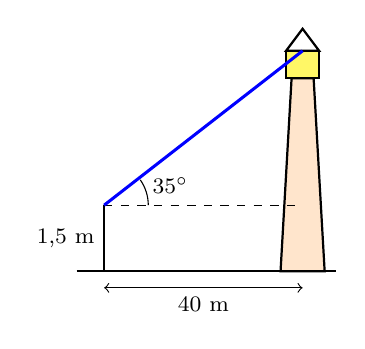
\begin{tikzpicture}[scale=0.7]
  % Mặt đất
  \draw[thick] (-0.5,0) -- (4.2,0);
  % Ngọn hải đăng
  \draw[thick, fill=orange!20] (3.2,0) -- (3.4,3.5) -- (3.8,3.5) -- (4.0,0) -- cycle;
  \draw[thick, fill=yellow!60] (3.3,3.5) rectangle (3.9,4.0);
  \draw[thick] (3.3,4.0) -- (3.6,4.4) -- (3.9,4.0) -- cycle;
  % Điểm quan sát và máy ngắm
  \draw[thick] (0,0) -- (0,1.2);
  \node[left] at (0,0.6) {\footnotesize $1{,}5\text{ m}$};
  \draw[dashed] (0,1.2) -- (3.5,1.2);
  \draw[thick, blue, line width=1.1pt] (0,1.2) -- (3.6,4.0);
  % Ký hiệu khoảng cách nằm ngang
  \draw[<->] (0,-0.3) -- (3.6,-0.3);
  \node[below] at (1.8,-0.3) {\footnotesize $40\text{ m}$};
  % Góc nâng 35 độ
  \draw (0,1.2) ++(0:0.8) arc (0:35:0.8);
  \node at (1.2,1.55) {\footnotesize $35^\circ$};
\end{tikzpicture}
\end{minipage}

\vspace{1.5mm}
\textbf{Câu 18.} Một bồn hoa hình quạt tròn có bán kính $R = 6\text{ m}$ và góc ở tâm tương ứng bằng $60^\circ$. Tính diện tích của bồn hoa đó (lấy $\pi \approx 3{,}14$, đơn vị: $\text{m}^2$).

\vspace{4mm}
\noindent
\textbf{\large II. TỰ LUẬN (3,0 điểm).} \textit{Thí sinh trình bày lời giải chi tiết vào tờ giấy thi.}

\vspace{2mm}
\textbf{Câu 19 (1,0 điểm).}
\begin{itemize}
  \item[a)] \textit{(0,5 điểm)} Giải hệ phương trình: $\begin{cases} 4x - 3y = 7 \\ 3x + 2y = 1 \end{cases}$.
  \item[b)] \textit{(0,5 điểm)} Cho biểu thức $B = \left( \dfrac{\sqrt{x}}{\sqrt{x}-3} - \dfrac{3}{\sqrt{x}+3} \right) : \dfrac{x+9}{x-9}$ với $x \ge 0, x \ne 9$. Rút gọn biểu thức $B$.
\end{itemize}

\vspace{2mm}
\textbf{Câu 20 (1,5 điểm).} Cho đường tròn $(O; R)$, đường kính $AB$. Lấy điểm $M$ bất kỳ trên $(O)$ ($M \ne A, B$). Tiếp tuyến tại $M$ cắt các tiếp tuyến tại $A$ và $B$ của $(O)$ lần lượt ở $C$ và $D$.
\begin{itemize}
  \item[a)] \textit{(0,75 điểm)} Chứng minh rằng $CD = AC + BD$ và $\widehat{COD} = 90^\circ$.
  \item[b)] \textit{(0,75 điểm)} Chứng minh rằng $AC \cdot BD = R^2$ và đường tròn đường kính $CD$ tiếp xúc với đường thẳng $AB$.
\end{itemize}

\vspace{2mm}
\textbf{Câu 21 (0,5 điểm).}
\begin{itemize}
  \item[a)] \textit{(0,25 điểm)} Bác Ba muốn làm một bể chứa nước bằng tôn dạng hình trụ không có nắp đậy với thể tích $V = 27\pi\text{ m}^3$. Hỏi bán kính đáy $R$ và chiều cao $h$ bằng bao nhiêu mét để lượng tôn dùng làm bể (diện tích toàn phần không nắp) là nhỏ nhất?
  \item[b)] \textit{(0,25 điểm)} Cho hai số thực dương $x, y$ thỏa mãn điều kiện $x + y = 2$. Tìm giá trị nhỏ nhất của biểu thức:
  \[
  P = \dfrac{1}{x^2 + y^2} + \dfrac{1}{xy}.
  \]
\end{itemize}

\vspace{4mm}
\begin{center}
\textbf{---------- HẾT ----------}\\
\textit{(Cán bộ coi thi không giải thích gì thêm)}
\end{center}

\end{document}
